\documentclass{article}

\usepackage[utf8]{inputenc}
\usepackage[T1]{fontenc}
\usepackage{graphicx}
\usepackage{booktabs}

\usepackage{Sweave}
\begin{document}
\Sconcordance{concordance:Informe.tex:Informe.Rnw:1 7 1 1 0 8 1 1 19 144 1 1 73 1 3 %
55 1 1 43 1 3 32 1}


\title{Informe técnico: análisis de Gapminder}
\author{A. Palomar}
\date{2 de septiembre de 2026}

\maketitle


\section{Introducción}

Este informe presenta el análisis de diferentes indicadores socioeconómicos
y demográficos a nivel mundial durante el periodo 1990--2019, utilizando
datos procedentes de Gapminder.

El análisis se centra en cuatro indicadores principales:

\begin{itemize}
    \item PIB per cápita.
    \item Esperanza de vida.
    \item Población.
    \item Hijos por mujer.
\end{itemize}

El objetivo del proyecto es analizar la evolución de estos indicadores
y estudiar las relaciones existentes entre ellos.

\section{Objetivos}

\subsection{Objetivo principal}

Analizar la evolución y la relación entre diferentes indicadores
socioeconómicos y demográficos a nivel mundial durante el periodo
1990--2019, utilizando datos de Gapminder.

\subsection{Objetivos específicos}

\begin{enumerate}

\item Analizar la evolución temporal de la esperanza de vida,
el PIB per cápita, la fertilidad y la población.

\item Estudiar la relación entre el PIB per cápita y la esperanza de vida.

\item Analizar la relación entre la fertilidad y la esperanza de vida.

\item Estudiar la relación entre el PIB per cápita y la fertilidad.

\item Comparar los indicadores entre los diferentes territorios.

\end{enumerate}

\section{Datos y metodología}

\subsection{Fuente de los datos}

Los datos utilizados en este proyecto proceden de Gapminder, una
organización que proporciona datos estadísticos sobre diferentes aspectos
del desarrollo económico y social a nivel mundial.

Para realizar el análisis se partió de cuatro bases de datos,
correspondientes a los diferentes indicadores seleccionados para el
proyecto. Estas bases de datos fueron integradas para obtener un único
conjunto de datos que permitiera analizar conjuntamente las variables
socioeconómicas y demográficas.

\subsection{Descripción de los datos}

La base de datos utilizada contiene
193 territorios y abarca desde el año
1990 hasta el año
2019.

Para el análisis se han seleccionado cuatro indicadores principales:

\begin{itemize}

    \item \textbf{PIB per cápita (GDP per capita):} indicador utilizado
    para aproximar el nivel económico de los territorios.

    \item \textbf{Esperanza de vida (Life expectancy):} número medio de
    años que se espera que viva una persona.

    \item \textbf{Población (Population):} número de habitantes de cada
    territorio.

    \item \textbf{Hijos por mujer (Babies per woman):} número medio de
    hijos por mujer, utilizado como indicador de fertilidad.

\end{itemize}

\subsection{Preparación de los datos}

Las cuatro bases de datos originales fueron revisadas y posteriormente
integradas en una única base de datos. A continuación, se realizó un
proceso de depuración para obtener un conjunto de datos final preparado
para el análisis.

La base de datos depurada constituye la fuente común utilizada para la
elaboración de las tablas, gráficos y análisis incluidos en este informe
y en el dashboard.

\subsection{Análisis exploratorio y visualización}

Como paso previo al desarrollo del dashboard se realizó un análisis
exploratorio de los datos (EDA). Este análisis permitió estudiar la
distribución de las variables, su evolución temporal y las relaciones
existentes entre los principales indicadores.

A partir de los resultados obtenidos en el EDA se diseñó un dashboard
interactivo que permite explorar visualmente los indicadores seleccionados
y sus relaciones. El dashboard incorpora diferentes gráficos y controles
interactivos que permiten seleccionar años, países e indicadores,
facilitando la comparación entre territorios y la identificación de
patrones.

\subsection{Metodología de análisis}

El análisis combina el estudio de la evolución temporal de los indicadores
con el análisis de las relaciones entre ellos.

En primer lugar, se estudia la evolución de la esperanza de vida, el PIB
per cápita, la población y la fertilidad durante el periodo 1990--2019.
Posteriormente, se analizan las relaciones entre el PIB per cápita y la
esperanza de vida, entre la fertilidad y la esperanza de vida, y entre el
PIB per cápita y la fertilidad.

Finalmente, se comparan los indicadores entre diferentes territorios para
identificar diferencias en sus características socioeconómicas y
demográficas.

\section{Resultados}

El análisis de los datos permite identificar diferentes patrones en la
evolución de los indicadores socioeconómicos y demográficos y en las
relaciones existentes entre ellos. Los resultados se presentan en
relación con los objetivos específicos definidos para el proyecto.


Los resultados mostrados en este informe constituyen una selección de los
principales análisis realizados. El dashboard desarrollado como parte del
proyecto permite explorar estos indicadores de forma interactiva,
seleccionando diferentes años y visualizando las relaciones entre ellos.

\subsection{Evolución temporal de los indicadores}

El análisis temporal permite observar cómo han evolucionado el PIB per
cápita, la esperanza de vida, la población y el número de hijos por mujer
durante el periodo 1990--2019.

A partir de la visualización de los datos se puede estudiar la tendencia
seguida por cada uno de estos indicadores.

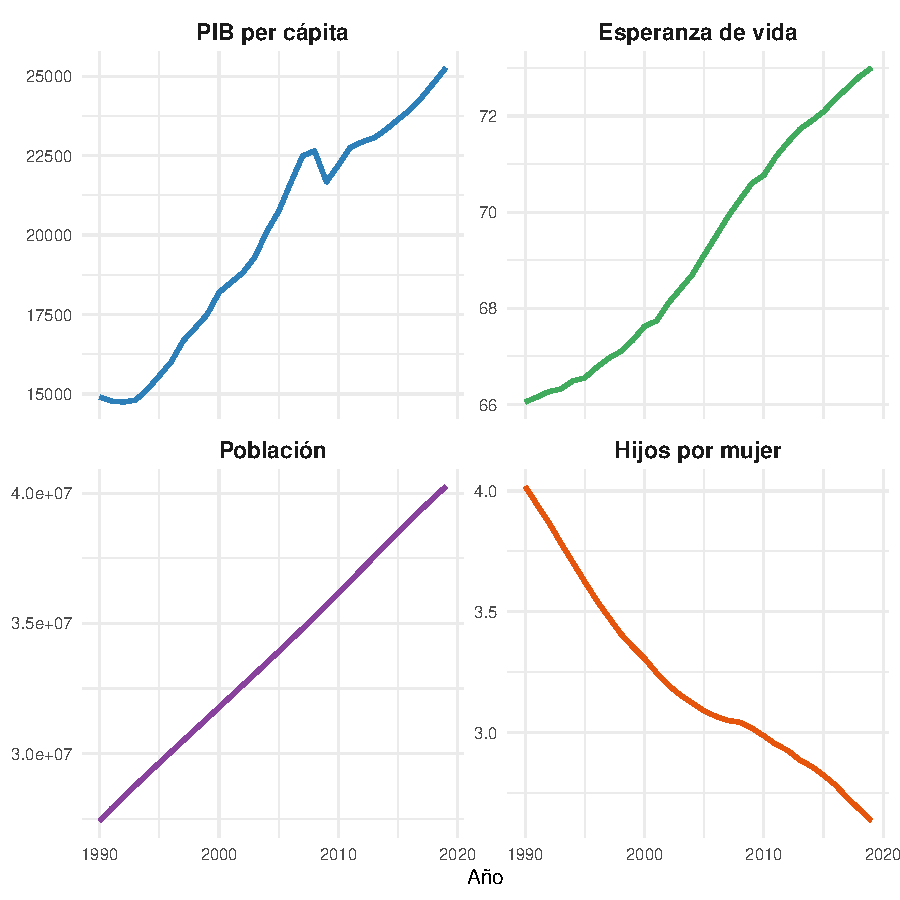
\includegraphics{Informe-grafico-evolucion}

La evolución temporal muestra tendencias diferenciadas entre los cuatro
indicadores. Entre 1990 y 2019, el PIB per cápita y la esperanza de vida
presentan una tendencia general creciente. La población también aumenta
de forma sostenida durante todo el periodo, mientras que el número de
hijos por mujer muestra una tendencia claramente descendente.

Estos resultados permiten observar una mejora general de algunos
indicadores socioeconómicos y demográficos, junto con una reducción de
la fertilidad. No obstante, estas tendencias corresponden a valores
medios y pueden ocultar diferencias importantes entre los distintos
territorios.

\begin{table}[h]
\centering
\caption{Evolución de los indicadores entre 1990 y 2019}
\begin{tabular}{lrr}
\toprule
Indicador & 1990 & 2019 \\
\midrule
PIB per cápita &
14906 &
25261 \\

Esperanza de vida &
66.1 &
73 \\

Población &
27421915 &
40257334 \\

Hijos por mujer &
4.02 &
2.64 \\

\bottomrule
\end{tabular}
\end{table}

La tabla muestra que entre 1990 y 2019 la esperanza de vida,
el PIB per cápita y la población presentan un incremento,
mientras que el número medio de hijos por mujer disminuye.

\subsection{Relación entre las variables}

Para analizar conjuntamente los principales indicadores se utiliza un
gráfico de burbujas. El PIB per cápita se representa en el eje horizontal
y la esperanza de vida en el eje vertical. El tamaño de las burbujas
representa la población, mientras que el color representa el número de
hijos por mujer.

En el dashboard, esta visualización puede explorarse de forma interactiva
seleccionando diferentes años. Para este informe se muestra el año 2019,
correspondiente al último año del periodo analizado.

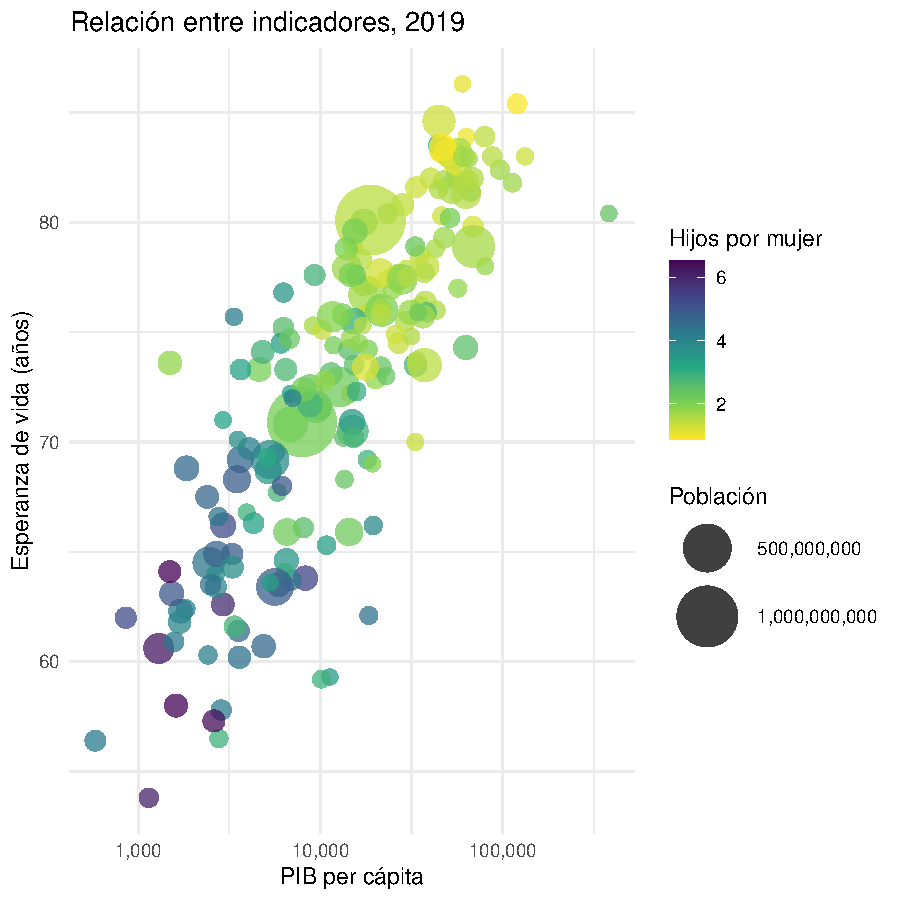
\includegraphics{Informe-grafico-burbujas}

El gráfico muestra una relación positiva entre el PIB per cápita y la
esperanza de vida. En general, los territorios con mayores niveles de
PIB per cápita presentan también una mayor esperanza de vida.

Además, los valores más elevados de hijos por mujer se concentran
principalmente entre los territorios con menores niveles de PIB per
cápita y esperanza de vida. El tamaño de las burbujas permite observar
también las diferencias de población entre los territorios.

\section{Conclusiones}

El análisis realizado permite identificar una evolución favorable de los
principales indicadores socioeconómicos y demográficos durante el periodo
1990--2019. La esperanza de vida, el PIB per cápita y la población
presentan una tendencia creciente, mientras que el número de hijos por
mujer disminuye.

El análisis de las relaciones entre variables muestra una asociación
positiva entre el PIB per cápita y la esperanza de vida. Asimismo, los
territorios con mayores niveles de fertilidad tienden a presentar menores
niveles de PIB per cápita y de esperanza de vida.

Finalmente, se observan diferencias importantes entre territorios en
los indicadores analizados. El dashboard permite ampliar estas
comparaciones mediante la selección interactiva de diferentes años y
territorios.

En conjunto, los resultados obtenidos permiten cumplir los objetivos
planteados y muestran la utilidad de la visualización interactiva para
explorar las relaciones entre los indicadores de Gapminder.

\end{document}
